\chapter{Evaluation}
\label{chapter:evaluation}

% \definecolor{win}{HTML}{0de929}
% \definecolor{loss}{HTML}{ef4748}
\definecolor{win}{HTML}{63be7b}
\definecolor{loss}{HTML}{f8696b}

TODO:

definition der testszenarien (was vergleichen wir, warum, wie)

hier ersteinmal leichte Vergleiche (z.B. greedy, random)

\begin{figure}[!ht]
    \centering
    \resizebox{\textwidth}{!}{\begin{tikzpicture}
            \coordinate (bar1Start) at (0,0);
            \coordinate (bar1End) at (10,0);
            \coordinate (bar1Break) at (2.1,0);

            \draw[color=win, line width=0.25cm] (bar1Start) -- (bar1Break);
            \draw[color=loss, line width=0.25cm] (bar1Break) -- (bar1End);
            \node[left = 0.1cm of bar1Start] {Random Player};
            \node[right = 0.1cm of bar1End, align=left] {Greedy Player \\ (eval: static)};
            \node[above right = 0.05cm and -0.15cm of bar1Start] {\footnotesize $21$ Gewonnen};
            \node[below = 0.1cm of bar1Break] {\scriptsize $21\%$};
            \node[above left = 0.05cm and -0.15cm of bar1End] {\footnotesize $79$ Verloren};
        \end{tikzpicture}}
    % \vspace*{-0.5cm}
    \caption{Rnadom Player vs. Greedy Player}
    \label{fig:random-greedy-comparison}
\end{figure}

TODO:

\section{Vergleich der PVS-Varianten}

TODO:

% ┌───────────────────────────── Principal Variation Search Player ─────────────────────────────┐
% │ Features:            [AW, TT(S), LMR, LMP, SE]                                              │
% │ Depth:               9 started from (P1: 11, P2: 13, type: Normal)                            │
% │ Time:                5.0634892s                                                             │
% │ Nodes searched:      43720                                                                  │
% │ Branching factor:    2.84 AVG / 1.78 EFF / 1.38 MEAN                                        │
% │ Best Action:         P7I1═4‖3↻1↔0P1 (0 pts)                                                 │
% │ Move Ordering:       86.80\% (8611 high pv / 9920 high)                                      │
% │ Aspiration window:   0 low / 0 high                                                         │
% │ Zero window search:  2 fails (0.01\%)                                                        │
% │ Search Extensions:   0 SP, 0 ST (enabled)                                                   │
% │ LMR (Fail/All):      0/114 (0.00%)                                                          │
% │ LMP:                 3271                                                                   │
% │ Principal Variation: P7I1═4‖3↻1↔0P1 → P21I0═2‖1↻0↔0P0 → P31I0═7‖4↻0↔1P1 → P11I0═0‖2↻0↔1P0 │
% │ ┌──────────────────────────── Transposition Table Statistics ─────────────────────────────┐ │
% │ │ Capacity:            10416666                                                           │ │
% │ │ Entries:              5257801 /  50.47\% filled                                          │ │
% │ │ Overwrites:          13138704                                                           │ │
% │ │ Accesses:             1141676                                                           │ │
% │ │ ├──► Hit:              261862 /  22.94\%                                                 │ │
% │ │ └──► Miss:             879814 /  77.06\%                                                 │ │
% │ └─────────────────────────────────────────────────────────────────────────────────────────┘ │
% └─────────────────────────────────────────────────────────────────────────────────────────────┘
\begin{figure}[!ht]
    \centering
    \resizebox{\textwidth}{!}{\begin{tcolorbox}[
                rounded corners=all,
                boxrule=1pt,
                colback=white,
                colframe=black,
                hbox,
                % width=\linewidth,
                enhanced,
                coltitle=black,
                title={\acl{PVS} Player},
                top=6pt,
                left=0pt,
                right=5pt,
                bottom=0pt,
                attach boxed title to top center={yshift=-\tcboxedtitleheight/2},
                boxed title style={size=small,colback=white,colframe=white}
            ]
            \begingroup
            \setlength{\arrayrulewidth}{0pt}

            \begin{tabular}{@{}ll@{}}
                Features:             & [AW, TT(S), \acs{LMR}, \acs{LMP}, SE]                                \\
                Depth:                & $9$ started from (P1: $11$, P2: $13$, type: Normal)                  \\
                Time:                 & $5{,}0634892\acs{s}$                                                 \\
                Nodes searched:       & $43720$                                                              \\
                Branching factor:     & $2{,}84$ AVG / $1{,}78$ EFF / $1{,}38$ MEAN                          \\
                Best Action:          & P7I1═4‖3↻1↔0P1 ($0$ pts)                                             \\
                Action Ordering:      & $86{,}80\%$ ($8611$ high pv / $9920$ high)                           \\
                Aspiration window:    & $0$ low / $0$ high                                                   \\
                Zero window search:   & $2$ fails ($0{,}01\%$)                                               \\
                Search Extensions:    & $0$ SP, $0$ ST (enabled)                                             \\
                \acs{LMR} (Fail/All): & $0/114$ ($0{,}00\%$)                                                 \\
                \acs{LMP}:            & $3271$                                                               \\
                \acl{PV}:             & P7I1═4‖3↻1↔0P1 → P21I0═2‖1↻0↔0P0 → P31I0═7‖4↻0↔1P1 → P11I0═0‖2↻0↔1P0 \\
                \multicolumn{2}{@{}c@{}}{
                \begin{tcolorbox}[
                        rounded corners=all,
                        boxrule=1pt,
                        colback=white,
                        colframe=black,
                        width=1.325\linewidth,
                        enhanced,
                        coltitle=black,
                        title={Transposition Table},
                        top=6pt,
                        left=0pt,
                        right=0pt,
                        bottom=0pt,
                        attach boxed title to top center={yshift=-\tcboxedtitleheight/2},
                        boxed title style={size=small,colback=white,colframe=white}
                    ]
                    \begin{tabular}{ll}
                        Capacity:   & $10416666$                      \\
                        Entries:    & $5257801$ /  $50{,}47\%$ filled \\
                        Overwrites: & $13138704$                      \\
                        Accesses:   & $1141676$                       \\
                        ├──► Hit:   & $261862$ /  $22{,}94\%$         \\
                        └──► Miss:  & $879814$ /  $77{,}06\%$         \\
                    \end{tabular}
                \end{tcolorbox}
                }                                                                                            \\
            \end{tabular}
            \endgroup
        \end{tcolorbox}}
    \vspace*{-0.25cm}
    \caption[PVS-Suchstatistiken]{\acs{PVS}-Suchstatistiken}
    \label{fig:pvs-statistics}
\end{figure}

TODO:

\begin{figure}[!ht]
    \centering
    \resizebox{\textwidth}{!}{\begin{tikzpicture}
            % \coordinate (bar1Start) at (0,0);
            % \coordinate (bar1End) at (10,0);
            % \coordinate (bar1Break) at (6.4,0);

            % \draw[color=win, line width=0.25cm] (bar1Start) -- (bar1Break);
            % \draw[color=loss, line width=0.25cm] (bar1Break) -- (bar1End);
            % \node[left = 0.1cm of bar1Start] {Hard-Fail};
            % \node[right = 0.1cm of bar1End] {Soft-Fail};
            % \node[above right = 0.05cm and -0.15cm of bar1Start] {\footnotesize $64$ Gewonnen};
            % \node[below = 0.1cm of bar1Break] {\scriptsize $64\%$};
            % \node[above left = 0.05cm and -0.15cm of bar1End] {\footnotesize $36$ Verloren};

            \coordinate (bar2Start) at (0,0);
            \coordinate (bar2End) at (10,0);
            \coordinate (bar2Break) at (5.1,0);

            \draw[color=win, line width=0.25cm] (bar2Start) -- (bar2Break);
            \draw[color=loss, line width=0.25cm] (bar2Break) -- (bar2End);
            \node[left = 0.1cm of bar2Start] {AspirationWindow};
            \node[right = 0.1cm of bar2End] {Kein AspirationWindow};
            \node[above right = 0.05cm and -0.15cm of bar2Start] {\footnotesize $51$ Gewonnen};
            \node[below = 0.1cm of bar2Break] {\scriptsize $51\%$};
            \node[above left = 0.05cm and -0.15cm of bar2End] {\footnotesize $49$ Verloren};

            \coordinate (bar3Start) at (0,-1.5);
            \coordinate (bar3End) at (10,-1.5);
            \coordinate (bar3Break) at (5.4,-1.5);

            \draw[color=win, line width=0.25cm] (bar3Start) -- (bar3Break);
            \draw[color=loss, line width=0.25cm] (bar3Break) -- (bar3End);
            \node[left = 0.1cm of bar3Start] {Sucherweiterungen};
            \node[right = 0.1cm of bar3End] {Keine Sucherweiterungen};
            \node[above right = 0.05cm and -0.15cm of bar3Start] {\footnotesize $54$ Gewonnen};
            \node[below = 0.1cm of bar3Break] {\scriptsize $54\%$};
            \node[above left = 0.05cm and -0.15cm of bar3End] {\footnotesize $46$ Verloren};

            \coordinate (bar4Start) at (0,-3);
            \coordinate (bar4End) at (10,-3);
            \coordinate (bar4Break) at (5.3,-3);

            \draw[color=win, line width=0.25cm] (bar4Start) -- (bar4Break);
            \draw[color=loss, line width=0.25cm] (bar4Break) -- (bar4End);
            \node[left = 0.1cm of bar4Start] {\acs{LMR}, \acs{LMP}};
            \node[right = 0.1cm of bar4End] {Kein \acs{LMR}, \acs{LMP}};
            \node[above right = 0.05cm and -0.15cm of bar4Start] {\footnotesize $53$ Gewonnen};
            \node[below = 0.1cm of bar4Break] {\scriptsize $53\%$};
            \node[above left = 0.05cm and -0.15cm of bar4End] {\footnotesize $47$ Verloren};

            \coordinate (bar5Start) at (0,-4.5);
            \coordinate (bar5End) at (10,-4.5);
            \coordinate (bar5Break) at (5,-4.5);

            \draw[color=win, line width=0.25cm] (bar5Start) -- (bar5Break);
            \draw[color=loss, line width=0.25cm] (bar5Break) -- (bar5End);
            \node[left = 0.1cm of bar5Start] {Table Ordering};
            \node[right = 0.1cm of bar5End] {Static Eval Ordering};
            \node[above right = 0.05cm and -0.15cm of bar5Start] {\footnotesize $50$ Gewonnen};
            \node[below = 0.1cm of bar5Break] {\scriptsize $50\%$};
            \node[above left = 0.05cm and -0.15cm of bar5End] {\footnotesize $50$ Verloren};

            \coordinate (bar6Start) at (0,-6);
            \coordinate (bar6End) at (10,-6);
            \coordinate (bar6Break) at (4.1,-6);

            \draw[color=win, line width=0.25cm] (bar6Start) -- (bar6Break);
            \draw[color=loss, line width=0.25cm] (bar6Break) -- (bar6End);
            \node[left = 0.1cm of bar6Start] {Kein \acs{SMP}};
            \node[right = 0.1cm of bar6End] {Lazy \acs{SMP}};
            \node[above right = 0.05cm and -0.15cm of bar6Start] {\footnotesize $41$ Gewonnen};
            \node[below = 0.1cm of bar6Break] {\scriptsize $41\%$};
            \node[above left = 0.05cm and -0.15cm of bar6End] {\footnotesize $59$ Verloren};
        \end{tikzpicture}}
    % \vspace*{-0.5cm}
    \caption[Vergleich der PVS Varianten]{Vergleich der \acs{PVS} Varianten}
    \label{fig:pvs-comparision}
\end{figure}

TODO:

\pagebreak

\section{Vergleich der MCTS-Varianten}

Im diesen Abschnitt werden die einzelnen Varianten des \ac{MCTS} Spielers miteinander verglichen. Zuerst sind dabei alle Tree Policies sowie Evaluatoren in der Tabelle \ref{tabelle:mcts-policy-eval-comparision} aufgelistet. Dabei tritt jede Kombination gegen jede andere Kombination an. In den einzelnen Zellen ist das Ergebnis der Vergleichsspiele als Gewinnrate zwischen 0 und 1 aus Sicht des Zeilenspielers aufgetragen (So gewinnt beispielsweise \emph{\acs{UCT},Win} mit $56{,}2\%$ gegen \emph{\acs{UCT},Score}). Die Vergleichsspiele umfassen dabei immer 1000 Spiele mit je 2500 Iterationen pro \hyperref[text:ply]{\emph{Ply}}. Um möglichst vergleichbare Spiele sicherzustellen, werden keine Suchbäume wiederverwendet und es findet auch keine Parallelisierung der einzelnen \ac{MCTS} Varianten statt.

\begin{table}[H]
    \centering
    \resizebox{\textwidth}{!}{\begin{tabular}{|c|c|c|c|c|c|c|c|c|c|c|}
            \hline
            \multicolumn{1}{|c}{Policy}       & $\rightarrow$ & \ac{UCT}                          & \ac{UCT}                          & \ac{UCT}                          & Score                             & Score                             & Score                             & \tiny \makecell{Partial-                                                                                  \\Score}  & \tiny \makecell{Partial-\\Score}  & \tiny \makecell{Partial-\\Score}  \\ \cline{3-11}
            \multicolumn{1}{|c}{$\downarrow$} & Evaluator     & Win                               & Score                             & Static                            & Win                               & Score                             & Static                            & Win                               & Score                             & Static                            \\ \hline
            \ac{UCT}                          & Win           & $\diagup$                         & \cellcolor[HTML]{ece683}$0{,}562$ & \cellcolor[HTML]{67bf7c}$0{,}989$ & \cellcolor[HTML]{c5db81}$0{,}686$ & \cellcolor[HTML]{fee883}$0{,}490$ & \cellcolor[HTML]{85c87d}$0{,}894$ & \cellcolor[HTML]{f3e884}$0{,}541$ & \cellcolor[HTML]{f7e984}$0{,}526$ & \cellcolor[HTML]{82c77d}$0{,}902$ \\ \hline
            \ac{UCT}                          & Score         & \cellcolor[HTML]{feda80}$0{,}438$ & $\diagup$                         & \cellcolor[HTML]{68c07c}$0{,}984$ & \cellcolor[HTML]{cadc81}$0{,}673$ & \cellcolor[HTML]{fbea84}$0{,}516$ & \cellcolor[HTML]{7ec67d}$0{,}914$ & \cellcolor[HTML]{f7e984}$0{,}526$ & \cellcolor[HTML]{feea83}$0{,}499$ & \cellcolor[HTML]{85c87d}$0{,}894$ \\ \hline
            \ac{UCT}                          & Static        & \cellcolor[HTML]{f86b6b}$0{,}011$ & \cellcolor[HTML]{f86d6b}$0{,}016$ & $\diagup$                         & \cellcolor[HTML]{f8726c}$0{,}038$ & \cellcolor[HTML]{f86d6b}$0{,}018$ & \cellcolor[HTML]{fcb87a}$0{,}305$ & \cellcolor[HTML]{f86e6c}$0{,}021$ & \cellcolor[HTML]{f86c6b}$0{,}013$ & \cellcolor[HTML]{fcb87a}$0{,}304$ \\ \hline
            Score                             & Win           & \cellcolor[HTML]{fcba7a}$0{,}314$ & \cellcolor[HTML]{fcbe7b}$0{,}327$ & \cellcolor[HTML]{6fc27c}$0{,}962$ & $\diagup$                         & \cellcolor[HTML]{fdca7d}$0{,}374$ & \cellcolor[HTML]{a0d07f}$0{,}805$ & \cellcolor[HTML]{fcc07b}$0{,}335$ & \cellcolor[HTML]{fcc47c}$0{,}353$ & \cellcolor[HTML]{9dcf7f}$0{,}816$ \\ \hline
            Score                             & Score         & \cellcolor[HTML]{fceb84}$0{,}510$ & \cellcolor[HTML]{fee683}$0{,}484$ & \cellcolor[HTML]{69c07c}$0{,}982$ & \cellcolor[HTML]{d8e082}$0{,}626$ & $\diagup$                         & \cellcolor[HTML]{7ec67d}$0{,}915$ & \cellcolor[HTML]{f6e984}$0{,}531$ & \cellcolor[HTML]{fbea84}$0{,}516$ & \cellcolor[HTML]{80c77d}$0{,}909$ \\ \hline
            Score                             & Static        & \cellcolor[HTML]{f98470}$0{,}106$ & \cellcolor[HTML]{f97f6f}$0{,}086$ & \cellcolor[HTML]{c3da81}$0{,}695$ & \cellcolor[HTML]{fa9b74}$0{,}195$ & \cellcolor[HTML]{f97f6f}$0{,}085$ & $\diagup$                         & \cellcolor[HTML]{f98871}$0{,}123$ & \cellcolor[HTML]{f9806f}$0{,}092$ & \cellcolor[HTML]{fedf81}$0{,}457$ \\ \hline
            \tiny \makecell{Partial-                                                                                                                                                                                                                                                                                                                                                              \\Score} &           Win & \cellcolor[HTML]{fee081}$0{,}459$ & \cellcolor[HTML]{fee482}$0{,}474$ & \cellcolor[HTML]{6ac07c}$0{,}979$ & \cellcolor[HTML]{ccdd82}$0{,}665$ & \cellcolor[HTML]{fee282}$0{,}469$ & \cellcolor[HTML]{8aca7e}$0{,}877$ & $\diagup$                         & \cellcolor[HTML]{fbea84}$0{,}513$ & \cellcolor[HTML]{82c77d}$0{,}903$ \\ \hline
            \tiny \makecell{Partial-                                                                                                                                                                                                                                                                                                                                                              \\Score} &         Score & \cellcolor[HTML]{fee482}$0{,}474$ & \cellcolor[HTML]{ffeb84}$0{,}501$ & \cellcolor[HTML]{68c07c}$0{,}987$ & \cellcolor[HTML]{d2de82}$0{,}647$ & \cellcolor[HTML]{fee683}$0{,}484$ & \cellcolor[HTML]{80c77d}$0{,}908$ & \cellcolor[HTML]{fee783}$0{,}487$ & $\diagup$                         & \cellcolor[HTML]{7cc67d}$0{,}920$ \\ \hline
            \tiny \makecell{Partial-                                                                                                                                                                                                                                                                                                                                                              \\Score} &        Static & \cellcolor[HTML]{f9826f}$0{,}098$ & \cellcolor[HTML]{f98470}$0{,}106$ & \cellcolor[HTML]{c2da81}$0{,}696$ & \cellcolor[HTML]{fa9874}$0{,}184$ & \cellcolor[HTML]{f9806f}$0{,}091$ & \cellcolor[HTML]{f2e884}$0{,}543$ & \cellcolor[HTML]{f9826f}$0{,}097$ & \cellcolor[HTML]{f97d6e}$0{,}080$ & $\diagup$                         \\ \hline
        \end{tabular}}
    \vspace{3pt}
    \caption{Vergleich der \acs{MCTS} Policy und Evaluator Varianten}
    \label{tabelle:mcts-policy-eval-comparision}
\end{table}

Wie in Tabelle \ref{tabelle:mcts-policy-eval-comparision} zu sehen ist, sind viele der Varianten sehr vergleichbar. So gewinnt die \emph{\acs{UCT},Win} Variante beispielsweise gegen alle anderen Varianten außer \emph{Score,Score}. Die \emph{Score,Score} Variante hingegen verliert gegen die \emph{\acs{UCT},Score} Variante, die wiederrum gegen die \emph{\acs{UCT},Win} Variante verliert. Die einzigen Varianten, welche eine deutlich schlechtere Leistung erbringen ist \emph{Score,Win} und alle Varianten mit dem statischen Evaluator. Die \emph{Score,Win} Variante erzeugt innerhalb der Simulationsphase immer das Ergebnis $-1$ oder $1$. Auf Basis dieser zwei Werte erzeugt die Score-Tree-Policy eine Auswahl der Knoten innerhalb der Selektionsphase, was natürlich nicht sehr aussagekräftig ist, womit auch das schlechtere Abschneiden erklärt ist. Die statische Evaluation wurde nur eingesetzt, weil es möglich ist. Jedoch wiederspricht diese statische Evaluation gerade dem Prinzip, wodurch der \ac{MCTS} Spieler seine Stärke erreicht: Möglichst viele Iterationen durchführen, um somit den wahren Wert einer Aktion durch eine genügend große Stichprobe an Spielverläufen ausreichend gut zu approximieren. Der statische Evaluator bricht den Vorgang verführt ab, um die Stichproben durch eine immer gleichbleibende und verzerrte Evaluation zu ersetzen. Somit ähnelt diese Variante eher dem \ac{PVS} Spieler der nur ein paar Ebenen tief schauen kann und schneidet deutlich schlechter ab, als die tatsächlichen \ac{MCTS} Varianten. Die tatsächlichen Varianten sind aber recht ähnlich. Aus diesem Grund wurde die \emph{Partial-Score} Tree Policy auch nur einmal mit $\rho = 10\%$ in die Tabelle mit aufgenommen. Nachfolgend wird deshalb auch einfach zufällig die \emph{\acs{UCT},WIn} Variante für die Vergleiche weiterverwendet .

\begin{figure}[!ht]
    \centering
    \begin{tikzpicture}
        \coordinate (bar1Start) at (0,0);
        \coordinate (bar1End) at (10,0);
        \coordinate (bar1Break) at (5,0);

        \draw[color=win, line width=0.25cm] (bar1Start) -- (bar1Break);
        \draw[color=loss, line width=0.25cm] (bar1Break) -- (bar1End);
        \node[left = 0.1cm of bar1Start] {Tree New};
        \node[right = 0.1cm of bar1End] {Tree Reuse};
        \node[above right = 0.05cm and -0.15cm of bar1Start] {\footnotesize $500$ Gewonnen};
        \node[below = 0.1cm of bar1Break] {\scriptsize $50\%$};
        \node[above left = 0.05cm and -0.15cm of bar1End] {\footnotesize $500$ Verloren};
    \end{tikzpicture}
    % \vspace*{-0.5cm}
    \caption[Vergleich Baumwiederverwendung bei MCTS]{Vergleich neuer Baum vs. Baum wiederverwenden bei \acs{MCTS}}
    \label{fig:mcts-tree-reuse-comparision}
\end{figure}

Weiterhin wird der \ac{MCTS} Spieler noch vergleichen, indem ein Spieler immer wieder versucht den alten Suchbaum wiederzuverwenden (\emph{Tree Reuse}, während der andere Spieler einfach direkt mit einem neuen Suchbaum anfängt (\emph{Tree New}). Das Ergebnis der 1000 Vergleichsspiele, bei dem jeder Spieler je 5000 Iterationen pro \hyperref[text:ply]{\emph{Ply}} zusteht, ist relativ ernüchternd. Wie in \ref{fig:mcts-tree-reuse-comparision} zu sehen ist, liegt das Ergebnis bei genau 50\% Gewinnrate beider Spieler. Möglicherweise kann das Ergebnis für \emph{Tree Reuse} noch verbessert werden, wenn mehr Iterationen gespielt werden, da dort ein größerer vorheriger Suchbaum existiert, jedoch sind hierfür noch umfangreichere Tests erforderlich.

\begin{figure}[!ht]
    \centering
    \begin{tikzpicture}
        \coordinate (bar1Start) at (0,0);
        \coordinate (bar1End) at (10,0);
        \coordinate (bar1Break) at (7.7,0);

        \draw[color=win, line width=0.25cm] (bar1Start) -- (bar1Break);
        \draw[color=loss, line width=0.25cm] (bar1Break) -- (bar1End);
        \node[left = 0.1cm of bar1Start, align=right] {\acs{MCTS}\\(1 Thread)};
        \node[right = 0.1cm of bar1End, align=left] {\acs{MCTS}\\(8 Leaf)};
        \node[above right = 0.05cm and -0.15cm of bar1Start] {\footnotesize $77$ Gewonnen};
        \node[below = 0.1cm of bar1Break] {\scriptsize $77\%$};
        \node[above left = 0.05cm and -0.15cm of bar1End] {\footnotesize $23$ Verloren};

        \coordinate (bar2Start) at (0,-1.5);
        \coordinate (bar2End) at (10,-1.5);
        \coordinate (bar2Break) at (4.6,-1.5);

        \draw[color=win, line width=0.25cm] (bar2Start) -- (bar2Break);
        \draw[color=loss, line width=0.25cm] (bar2Break) -- (bar2End);
        \node[left = 0.1cm of bar2Start, align=right] {\acs{MCTS}\\(1 Thread)};
        \node[right = 0.1cm of bar2End, align=left] {\acs{MCTS}\\(8 Root)};
        \node[above right = 0.05cm and -0.15cm of bar2Start] {\footnotesize $46$ Gewonnen};
        \node[below = 0.1cm of bar2Break] {\scriptsize $46\%$};
        \node[above left = 0.05cm and -0.15cm of bar2End] {\footnotesize $54$ Verloren};

        \coordinate (bar3Start) at (0,-3);
        \coordinate (bar3End) at (10,-3);
        \coordinate (bar3Break) at (1.8,-3);

        \draw[color=win, line width=0.25cm] (bar3Start) -- (bar3Break);
        \draw[color=loss, line width=0.25cm] (bar3Break) -- (bar3End);
        \node[left = 0.1cm of bar3Start, align=right] {\acs{MCTS}\\(8 Leaf)};
        \node[right = 0.1cm of bar3End, align=left] {\acs{MCTS}\\(8 Root)};
        \node[above right = 0.05cm and -0.15cm of bar3Start] {\footnotesize $18$ Gewonnen};
        \node[below = 0.1cm of bar3Break] {\scriptsize $18\%$};
        \node[above left = 0.05cm and -0.15cm of bar3End] {\footnotesize $82$ Verloren};
    \end{tikzpicture}
    % \vspace*{-0.5cm}
    \caption[Vergleich der MCTS Varianten]{Vergleich der \acs{MCTS} Varianten}
    \label{fig:mcts-comparision}
\end{figure}

Um die \ac{MCTS} Spielervergleiche abzuschließen, werden zuletzt die einzelnen Parallelisierungsmöglichkeiten untereinander in \ref{fig:mcts-comparision} verglichen. Dabei spielen die nicht parallelisierte Single-Threaded Variante sowie die Leaf- und Root-Parallelisierten Varianten mit 8 Threads gegenaeinander. Die \hyperref[text:leaf-parallelization]{\emph{Leaf Parallelisierung}} schneidet dabei am schlechtesten ab, auch schlechter als die \ac{MCTS} Suche mit einem Thread. Da der \ac{MCTS} Spieler in Patchwork generell sehr wenige Iterationen schafft, ist es wahrscheinlich besser die Change einen guten Spielverlauf zu finden durch viele Iterationen zu maximieren, anstatt weniger Pfade auszuprobieren und für diese Pfade mittels \hyperref[text:leaf-parallelization]{\emph{Leaf Parallelisierung}} eine etwas genaueren Schätzer für den tatsächlichen Wert eines Knotens zu erhalten. Am besten spielt die \hyperref[text:root-parallelization]{\emph{Root-Parallelisierte}} Variante. Diese setzt sich gegen beide anderen Varianten durch, auch wenn der Vorsprung vor der Single-Threaded Variante geringer ausfällt als erhofft.

% ┌───────────────────────────── MCTS Player ─────────────────────────────┐
% │ Features:            [RP(8), RT]                                      │
% │ Duration:            9.925s                                           │
% │ Total Iterations:    592082                                           │
% │ Iterations:          74767                                            │
% │ Nodes:               74791                                            │
% │ Reused Tree:         true                                             │
% │ Root actions:        110                                              │
% │ Expanded Depth:      4                                                │
% │ Win Percentage:      98.40%                                           │
% │ Principal Variation: P17I2═5‖0↻0↔0P1 → W27 → P28I0═8‖1↻0↔0P1 → S═4‖4 │
% │ Min/Max Evaluation:  -1/1                                             │
% └───────────────────────────────────────────────────────────────────────┘
\begin{figure}[!ht]
    \centering
    \resizebox{\textwidth}{!}{\begin{tcolorbox}[
                rounded corners=all,
                boxrule=1pt,
                colback=white,
                colframe=black,
                hbox,
                % width=\linewidth,
                enhanced,
                coltitle=black,
                title={\acs{MCTS} Player},
                top=6pt,
                left=0pt,
                right=3pt,
                bottom=0pt,
                attach boxed title to top center={yshift=-\tcboxedtitleheight/2},
                boxed title style={size=small,colback=white,colframe=white}
            ]
            \begingroup
            \setlength{\arrayrulewidth}{0pt}

            \begin{tabular}{@{}ll@{}}
                Features:           & [RP(8), RT]                                     \\
                Duration:           & $9{,}925\acs{s}$                                \\
                Total Iterations:   & $592082$                                        \\
                Iterations:         & $74767$                                         \\
                Nodes:              & $74791$                                         \\
                Reused Tree:        & true                                            \\
                Root actions:       & $110$                                           \\
                Expanded Depth:     & $4$                                             \\
                Win Percentage:     & $98{,}40\%$                                     \\
                \acl{PV}:           & P17I2═5‖0↻0↔0P1 → W27 → P28I0═8‖1↻0↔0P1 → S═4‖4 \\
                Min/Max Evaluation: & $-1\ /\ 1$                                      \\
            \end{tabular}

            \endgroup
        \end{tcolorbox}}
    \vspace*{-0.25cm}
    \caption[MCTS-Suchstatistiken]{\acs{MCTS}-Suchstatistiken}
    \label{fig:mcts-statistics}
\end{figure}

Abschließend werden wie beim \ac{PVS} Spieler noch verschiedene Statistiken zu einer \ac{MCTS} Suche betrachtet. Die in Abbildung \ref{fig:mcts-statistics} gezeigte Auflistung stammt dabei von einem \ac{MCTS} Spieler mit einer \hyperref[text:root-parallelization]{\emph{Root Parallelisierung}} mit 8 Threads, der seinen Suchbaum wiederverwendet, die \ac{UCT} Tree Policy sowie den Win-Loss-Evaluator verwendet. Generell schafft ein Thread innerhalb der Suchzeit meistens zwischen $50{.}000$ und $100{.}000$ Iterationen. Je später im Spiel eine Aktion gesucht wird, desto mehr Iterationen sind es normalerweise, da eine Simulationsphase zum Beispiel statt $42$ nur noch $10$ \hyperref[text:ply]{\emph{Plys}} umfasst. Über eine Vielzahl von Iterationen summiert sich dieser kleine Zeitunterschied auf. In der dargestellten Auflistung hat der Main-Thread $74{.}767$ Iterationen geschafft. Es ist auch zu erkennen, dass die \hyperref[text:root-parallelization]{\emph{Root Parallelisierung}} einwandfrei funktioniert. Schafft ein Thread $74{.}767$ Iterationen, so müssten 8 Threads $74{.}767 \cdot 8 = 598{.}136$ Iterationen schaffen. Der tatsächliche Wert aller Threads liegt bei $592{.}082$ Iterationen, was einer prozentualen Abweichung von $-1{,}01\%$ vom erwarteten Wert entspricht und somit innerhalb der Fehlermarge liegt. Auch gibt es im Suchbaum des Main-Threads leicht weniger Knoten als Iterationen im Baum. Somit wurde die Expansionsphase innerhalb einiger Iterationen übersprungen, was nur vorkommen kann, falls ein Spielverlauf verfolgt wird, der im Baum in einem bereits bestehendem Terminalknoten endet. Das ist generell ein gutes Zeichen, da der \ac{MCTS} Spieler in diesem Fall bereit einen großen Bereich der möglichen Spielverläufe erkundet oder einen sehr vielversprechenden Spielverlauf gefunden hat. Die \acl{PV} ist 4 \hyperref[text:ply]{\emph{Plys}} lang. Somit wurden entlang der \ac{PV} vier Ebenen lang alle möglichen Aktionen expandiert und mindestens einmal erkunden. Nach diesen vier Ebenen existieren noch weitere Ebenen, bei denen aber noch nicht alle möglichen Aktionen erkunden sind.

\section{Evaluation von PatchZero}

TODO:

\begin{figure}[!ht]
    \centering
    \begin{tikzpicture}
        \coordinate (bar1Start) at (0,0);
        \coordinate (bar1End) at (10,0);
        \coordinate (bar1Break) at (5.5,0);

        \draw[color=win, line width=0.25cm] (bar1Start) -- (bar1Break);
        \draw[color=loss, line width=0.25cm] (bar1Break) -- (bar1End);
        \node[left = 0.1cm of bar1Start] {PatchZero};
        \node[right = 0.1cm of bar1End] {RandomPlayer};
        \node[above right = 0.05cm and -0.15cm of bar1Start] {\footnotesize $55$ Gewonnen};
        \node[below = 0.1cm of bar1Break] {\scriptsize $55\%$};
        \node[above left = 0.05cm and -0.15cm of bar1End] {\footnotesize $45$ Verloren};

        \coordinate (bar2Start) at (0,-1.5);
        \coordinate (bar2End) at (10,-1.5);
        \coordinate (bar2Break) at (2.2,-1.5);

        \draw[color=win, line width=0.25cm] (bar2Start) -- (bar2Break);
        \draw[color=loss, line width=0.25cm] (bar2Break) -- (bar2End);
        \node[left = 0.1cm of bar2Start] {PatchZero};
        \node[right = 0.1cm of bar2End] {GreedyPlayer};
        \node[above right = 0.05cm and -0.15cm of bar2Start] {\footnotesize $22$ Gewonnen};
        \node[below = 0.1cm of bar2Break] {\scriptsize $22\%$};
        \node[above left = 0.05cm and -0.15cm of bar2End] {\footnotesize $78$ Verloren};
    \end{tikzpicture}
    % \vspace*{-0.5cm}
    \caption{TODO:}
    \label{fig:patchzero-comparision}
\end{figure}

TODO:

\section{Paarvergleiche}

TODO:

\begin{figure}[!ht]
    \centering
    \resizebox{\textwidth}{!}{\begin{tikzpicture}
            \coordinate (bar1Start) at (0,0);
            \coordinate (bar1End) at (10,0);
            \coordinate (bar1Break) at (8.6,0);

            \draw[color=win, line width=0.25cm] (bar1Start) -- (bar1Break);
            \draw[color=loss, line width=0.25cm] (bar1Break) -- (bar1End);
            \node[left = 0.1cm of bar1Start, align = right] {\acs{PVS}-Player \\ (1 Thread)};
            \node[right = 0.1cm of bar1End] {RandomPlayer};
            \node[above right = 0.05cm and -0.15cm of bar1Start] {\footnotesize $86$ Gewonnen};
            \node[below = 0.1cm of bar1Break] {\scriptsize $86\%$};
            \node[above left = 0.05cm and -0.15cm of bar1End] {\footnotesize $14$ Verloren};

            \coordinate (bar2Start) at (0,-1.5);
            \coordinate (bar2End) at (10,-1.5);
            \coordinate (bar2Break) at (6.6,-1.5);

            \draw[color=win, line width=0.25cm] (bar2Start) -- (bar2Break);
            \draw[color=loss, line width=0.25cm] (bar2Break) -- (bar2End);
            \node[left = 0.1cm of bar2Start, align = right] {\acs{PVS}-Player \\ (1 Thread)};
            \node[right = 0.1cm of bar2End] {GreedyPlayer};
            \node[above right = 0.05cm and -0.15cm of bar2Start] {\footnotesize $66$ Gewonnen};
            \node[below = 0.1cm of bar2Break] {\scriptsize $66\%$};
            \node[above left = 0.05cm and -0.15cm of bar2End] {\footnotesize $34$ Verloren};
        \end{tikzpicture}}
    % \vspace*{-0.5cm}
    \caption[PVS Spieler vs. Random und Greedy]{\acs{PVS} Spieler vs. Random und Greedy}
    \label{fig:pvs-random-greedy-comparision}
\end{figure}

TODO:

\begin{figure}[!ht]
    \centering
    \resizebox{\textwidth}{!}{\begin{tikzpicture}
            \coordinate (bar1Start) at (0,0);
            \coordinate (bar1End) at (10,0);
            \coordinate (bar1Break) at (5,0);

            \draw[color=win, line width=0.25cm] (bar1Start) -- (bar1Break);
            \draw[color=loss, line width=0.25cm] (bar1Break) -- (bar1End);
            \node[left = 0.1cm of bar1Start, align=right] {\acs{MCTS}-Player \\ (1 Thread)};
            \node[right = 0.1cm of bar1End] {RandomPlayer};
            \node[above right = 0.05cm and -0.15cm of bar1Start] {\footnotesize $00$ Gewonnen};
            \node[below = 0.1cm of bar1Break] {\scriptsize $00\%$};
            \node[above left = 0.05cm and -0.15cm of bar1End] {\footnotesize $00$ Verloren};

            \coordinate (bar2Start) at (0,-1.5);
            \coordinate (bar2End) at (10,-1.5);
            \coordinate (bar2Break) at (5,-1.5);
            \draw[color=win, line width=0.25cm] (bar2Start) -- (bar2Break);
            \draw[color=loss, line width=0.25cm] (bar2Break) -- (bar2End);
            \node[left = 0.1cm of bar2Start, align=right] {\acs{MCTS}-Player \\ (1 Thread)};
            \node[right = 0.1cm of bar2End] {GreedyPlayer};
            \node[above right = 0.05cm and -0.15cm of bar2Start] {\footnotesize $00$ Gewonnen};
            \node[below = 0.1cm of bar2Break] {\scriptsize $00\%$};
            \node[above left = 0.05cm and -0.15cm of bar2End] {\footnotesize $00$ Verloren};
        \end{tikzpicture}}
    % \vspace*{-0.5cm}
    \caption[MCTS Spieler vs. Random und Greedy]{\acs{MCTS} Spieler vs. Random und Greedy}
    \label{fig:mcts-random-greedy-comparision}
\end{figure}

TODO:

\begin{figure}[!ht]
    \centering
    \begin{tikzpicture}
        \coordinate (bar1Start) at (0,0);
        \coordinate (bar1End) at (10,0);
        \coordinate (bar1Break) at (0.1,0);

        \draw[color=win, line width=0.25cm] (bar1Start) -- (bar1Break);
        \draw[color=loss, line width=0.25cm] (bar1Break) -- (bar1End);
        \node[left = 0.1cm of bar1Start, align=right] {\acs{PVS} Player \\ (1 Thread)};
        \node[right = 0.1cm of bar1End, align=left] {\acs{MCTS} Player \\ (1 Thread)};
        \node[above right = 0.05cm and -0.15cm of bar1Start] {\footnotesize $1$ Gewonnen};
        \node[below = 0.1cm of bar1Break] {\scriptsize $1\%$};
        \node[above left = 0.05cm and -0.15cm of bar1End] {\footnotesize $99$ Verloren};

        \coordinate (bar2Start) at (0,-1.5);
        \coordinate (bar2End) at (10,-1.5);
        \coordinate (bar2Break) at (0,-1.5);

        \draw[color=win, line width=0.25cm] (bar2Start) -- (bar2Break);
        \draw[color=loss, line width=0.25cm] (bar2Break) -- (bar2End);
        \node[left = 0.1cm of bar2Start, align=right] {\acs{PVS} Player \\ (8 Threads)};
        \node[right = 0.1cm of bar2End, align=left] {\acs{MCTS} Player \\ (1 Thread)};
        \node[above right = 0.05cm and -0.15cm of bar2Start] {\footnotesize $0$ Gewonnen};
        \node[below = 0.1cm of bar2Break] {\scriptsize $0\%$};
        \node[above left = 0.05cm and -0.15cm of bar2End] {\footnotesize $100$ Verloren};

        \coordinate (bar3Start) at (0,-3);
        \coordinate (bar3End) at (10,-3);
        \coordinate (bar3Break) at (0.1,-3);

        \draw[color=win, line width=0.25cm] (bar3Start) -- (bar3Break);
        \draw[color=loss, line width=0.25cm] (bar3Break) -- (bar3End);
        \node[left = 0.1cm of bar3Start, align=right] {\acs{PVS} Player \\ (8 Threads)};
        \node[right = 0.1cm of bar3End, align=left] {\acs{MCTS} Player \\ (8 Threads)};
        \node[above right = 0.05cm and -0.15cm of bar3Start] {\footnotesize $1$ Gewonnen};
        \node[below = 0.1cm of bar3Break] {\scriptsize $1\%$};
        \node[above left = 0.05cm and -0.15cm of bar3End] {\footnotesize $99$ Verloren};
    \end{tikzpicture}
    \caption{\acs{PVS} Player vs. \acs{MCTS} Player}
    \label{fig:pvs-mcts-comparison}
\end{figure}

TODO:

\begin{figure}[!ht]
    \centering
    \resizebox{\textwidth}{!}{\begin{tikzpicture}
            \coordinate (bar1Start) at (0,0);
            \coordinate (bar1End) at (10,0);
            \coordinate (bar1Break) at (3.1,0);

            \draw[color=win, line width=0.25cm] (bar1Start) -- (bar1Break);
            \draw[color=loss, line width=0.25cm] (bar1Break) -- (bar1End);
            \node[left = 0.1cm of bar1Start, align=right] {Greedy Player \\ (eval: static)};
            \node[right = 0.1cm of bar1End, align=left] {Greedy Player \\ (eval: score)};
            \node[above right = 0.05cm and -0.15cm of bar1Start] {\footnotesize $31$ Gewonnen};
            \node[below = 0.1cm of bar1Break] {\scriptsize $31\%$};
            \node[above left = 0.05cm and -0.15cm of bar1End] {\footnotesize $69$ Verloren};
        \end{tikzpicture}}
    % \vspace*{-0.5cm}
    \caption[Statische Evaluation vs. Score Evaluation]{Statische Evaluation vs. Random Rollout Score Evaluation}
    \label{fig:greedy-static-greedy-score-comparison}
\end{figure}

TODO:

\section{Platzierungen innerhalb des Glicko-2-Systems}

Auch wenn die einzelnen Paarvergleiche der Computerengines einen groben Einblick in die Leistungsfähigkeit der einzelnen Spieler geben können, ist ein präzises Ranking aller Spieler anschaulicher. Deshalb wird das Glicko-2-System verwendet, um einen genaueren Überblick sowie eine Einschätzung für ein präzises Ranking zu erstellen. Das Glicko-System ist ein mathematisches Bewertungssystem, das speziell für die Bewertung der Spielstärke von Spielern in Turnieren entwickelt wurde \cite[S. 377]{1999.GlickoMath}. Im originalen Glicko-System wird neben der genauen Bewertung auch eine \enquote{Rating Derviation} geschätzt \cite[S. 1f.]{2016.Glicko}. Die \enquote{Rating Derviation} entspricht der Standardabweichung und stellt die Unsicherheit bei der Schätzung der Bewertung dar. So kann neben dem Punktschätzer der Bewertung auch ein Konfidenzintervall angegeben werden, in dem die Bewertung eines Spielers mit einer hohen Wahrscheinlichkeit liegt. Das Glicko-2-System erweitert diese Modellierung noch um die \emph{Volatilität}, welche niedrig ist falls ein Spieler konstant gleiche Leistungen erbringt und hoch, wenn ein Spieler unregelmäßig größere Ausreißer in den Leistungen zeigt \cite[S. 1]{2022.Glicko2}. Das Glicko-2-System wird auch von Schachwebseiten wie \enquote{Lichess} für das Rating der Spieler verwendet, während andere Webseiten wie \enquote{Chess.com} den Vorgänger Glicko-1 verwenden \cite{2024.ChessRatingSystems}.

Für die Vergabe der Bewertung sind jedem Spieler zum Anfang die aus dem Glicko-2-Paper übernommenen Standardwerte von 1500 für die Bewertung, 350 für die \enquote{Rating Derviation} und $0{,}06$ für die \emph{Volatilität} zugeordnet \cite[S. 2]{2022.Glicko2}. Diese Werte werden dann inkrementell aktualisiert, indem die zuvor beschriebenen Vergleichsspiele als Ergebnisse eingesetzt werden. Die daraus entstehende Rangliste ist in Abbildung \ref{fig:player-ratings} dargestellt. Dabei werden bei den Spielern, welche mehrere Varianten besitzen, der Übersichtlichkeit halber immer nur die besten Varianten dargestellt.

\begin{figure}[!ht]
    \centering
    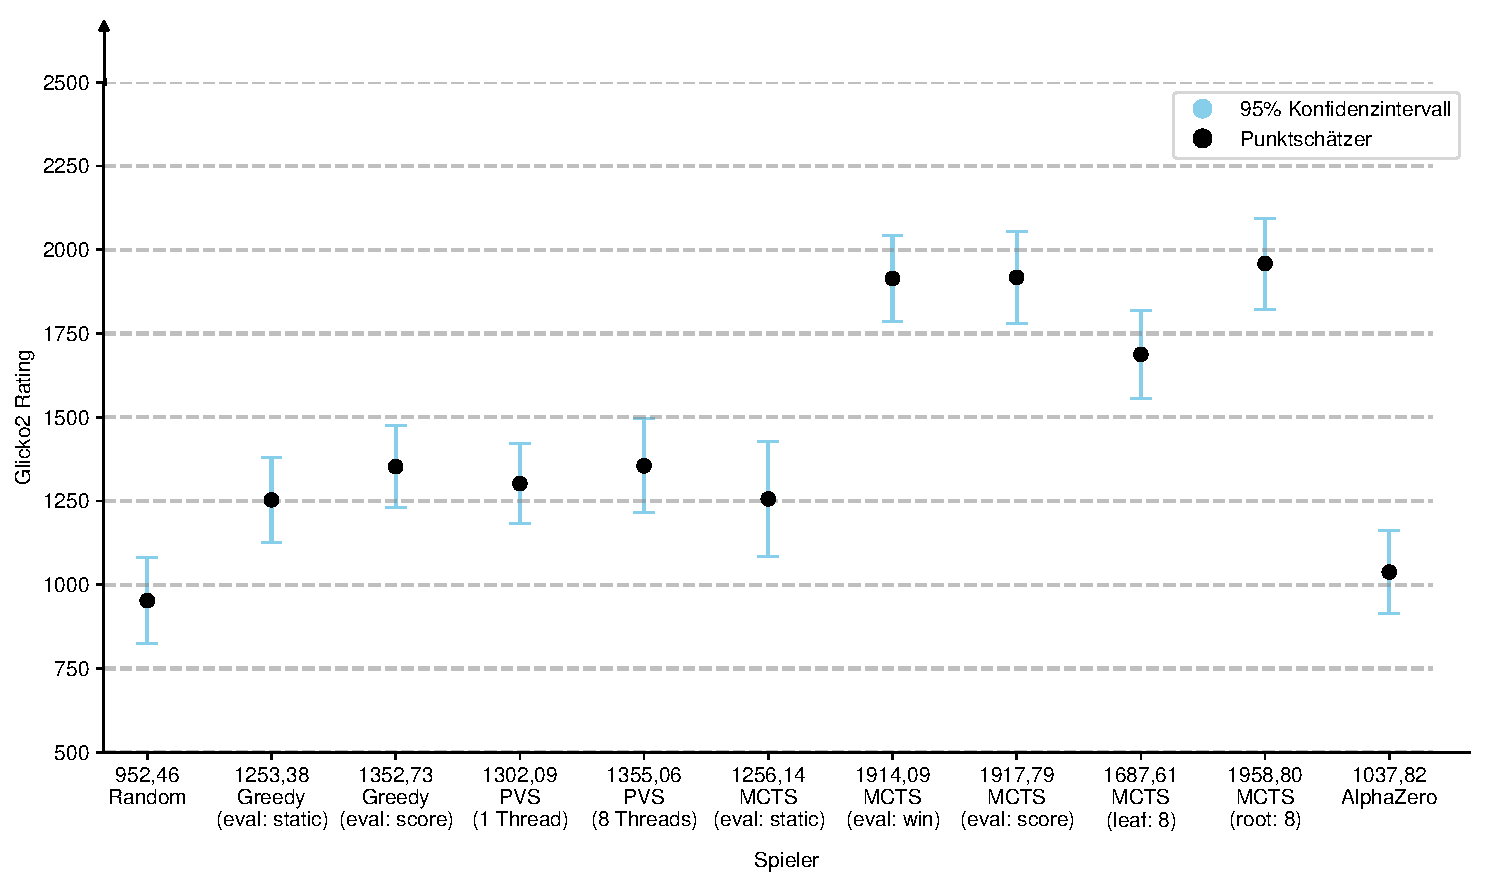
\includegraphics[width=\textwidth]{res/pictures/plots/player-ratings.pdf}
    \caption{Bewertung der Spieler im Glicko-2-Wertungssystem}
    \label{fig:player-ratings}
\end{figure}

In der Rangliste spiegeln sich die Ergebnisse der Vergleichspartien. Auch hier ist der RandomPlayer der schlechteste Spieler. Kurz davor liegt PatchZero. Die Greedy und \ac{PVS} Spieler Varianten teilen sich zusammen in eine ähnliche Bewertungsgruppe ein, wobei der mit Lazy \ac{SMP} parallelisierte \ac{PVS} Spieler die Gruppe anführt. Die \ac{MCTS} Varianten stehen deutlich von den anderen Spielern abgesetzt auf den vorderen Plätzen. Nur der \ac{MCTS} Spieler mit einer statischen Evaluation liegt im Bereich von Greedy- und \ac{PVS}-Spieler. Dies ist nicht verwunderlich, da diese Variante auch eher ähnlich zu diesen Spielern arbeitet, als wie die tatsächlichen \ac{MCTS} Spieler. Die \hyperref[text:leaf-parallelization]{\emph{Leaf Parallelisierung}} bei \ac{MCTS} liegt leicht abgeschlagen von den anderen Varianten, jedoch immer noch weit vor allen anderen Algorithmen, während \hyperref[text:root-parallelization]{\emph{Root Parallelisierung}} einen kleinen Rangvorsprung über die Single-Threaded \ac{MCTS} Varianten aufbauen kann. An dieser Stelle ist es wichtig anzumerken, dass alle in Abbildung \ref{fig:player-ratings} aufgezeigten Glicko-2-Ratings nur relativ zueinander sind und somit nicht mit anderen Glicko-2-Ratings, zum Beispiel von Schach, verglichen werden können.

TODO:

\section{Ergebnisse gegen die Autoren}

TODO: